%% Fig 7 -- regenerated by LIEP-REGEN (owner's OK 2026-11-05; revised 2026-11-13: one backprop control for every curve, linear axis; 2026-11-16: stage 4d grid, 31 cells x 8 draws, logit axis for the stuck fractions; 2026-11-17: each recovery panel's y range spans lock-in EP's results in that panel). DRAFT caption for the owner to edit into the manuscript.
%% Graphic: regen/figures/src/fig7_recovery.py, data and macros from regen/figures/export.py. Replaces fig2_recovery.
% generated by regen/figures/export.py -- do not edit
\newcommand{\FigClean}{0.8606}
\newcommand{\FigNdraw}{8}
\newcommand{\FigCeilLockin}{0.8706}
\newcommand{\FigCeilLockinLo}{0.8657}
\newcommand{\FigCeilLockinHi}{0.8724}
\newcommand{\FigCeilCentred}{0.8637}
\newcommand{\FigCeilCentredLo}{0.8588}
\newcommand{\FigCeilCentredHi}{0.8672}
\newcommand{\FigCeilBp}{0.8636}
\newcommand{\FigCeilBpLo}{0.8605}
\newcommand{\FigCeilBpHi}{0.8673}
\newcommand{\FigCeilRo}{0.8632}
\newcommand{\FigCeilRoLo}{0.8613}
\newcommand{\FigCeilRoHi}{0.8656}
\newcommand{\FigCeilN}{8}
\newcommand{\FigGTop}{24}
\newcommand{\FigGTopLockin}{0.435}
\newcommand{\FigGTopCentred}{0.663}
\newcommand{\FigGTopBp}{0.679}


\begin{figure}[tbp]
\sffamily
\centering
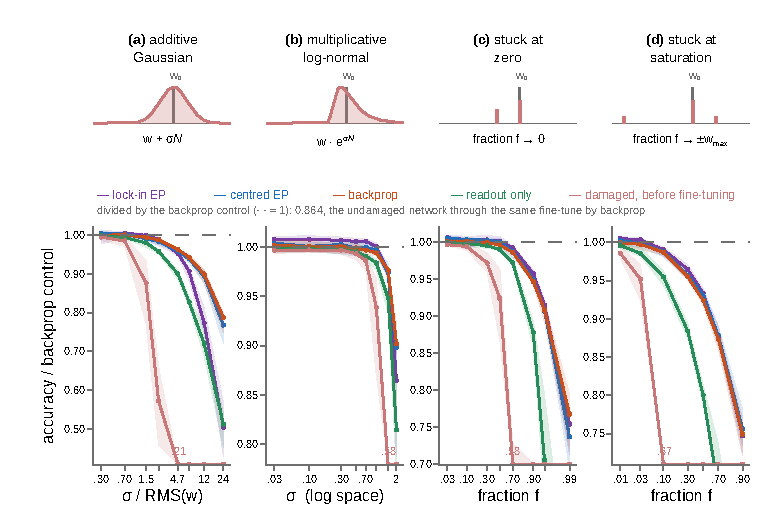
\includegraphics[width=\textwidth]{figures/fig7_recovery.pdf}
\caption{Analog weight distortion, and what recovers from it. One column per fault: \textbf{(a)} additive Gaussian
noise, \textbf{(b)} the multiplicative log-normal map, \textbf{(c)} weights stuck at zero, \textbf{(d)} weights stuck
at saturation. Above each column, the map applied to a single weight, drawn schematically. Below, test accuracy
(EP settle, 10,000 images) against severity after a backprop-pretrained network is damaged once and fine-tuned for
three epochs by each arm: lock-in EP, centred EP, backprop, and backprop into the readout layer only. Every arm sees the
same fault mask, and stuck devices stay stuck under every arm. Median of \FigNdraw{} damage draws, bands min--max.
Every curve is divided by one control, the undamaged network put through the same fine-tune by backprop
(\FigCeilBp; \FigCeilN{} draws; dashed line at 1). The other arms reach lock-in \FigCeilLockin, centred
\FigCeilCentred{} and readout-only \FigCeilRo{} on the undamaged network, so values slightly above 1 are within
fine-tuning noise. Each panel's vertical range spans lock-in EP's results under that fault; curves that fall below it leave
through the bottom edge. The damaged network before fine-tuning is divided by the same control and is drawn along the
bottom edge once it falls below the axis, with its value printed where it leaves. Severity axes are
logarithmic in (a) and (b) and logit-spaced in (c) and (d), so that stuck fractions up to 0.99 stay apart. Lock-in and
centred EP recover alike under every fault except strong additive noise: at $\sigma=\FigGTop\times$ the weights' RMS,
centred EP reaches \FigGTopCentred{}, close to backprop (\FigGTopBp), and lock-in EP \FigGTopLockin.}
\label{fig:repair}
\end{figure}
